\documentclass[a4paper,german]{scrreprt}

% Uncomment to optimize for double-sided printing.
% \KOMAoptions{twoside}

% Set binding correction manually, if known.
% \KOMAoptions{BCOR=2cm}

% Localization options
\usepackage[german]{babel}
\usepackage[T1]{fontenc}
\usepackage[utf8]{inputenc}

% Enhanced verbatim sections. We're mainly interested in
% \verbatiminput though.
\usepackage{verbatim}

% PDF-compatible landscape mode.
% Makes PDF viewers show the page rotated by 90°.
\usepackage{pdflscape}

% Advanced tables
\usepackage{tabu}
\usepackage{longtable}
\usepackage{dcolumn}
\newcolumntype{d}[1]{D{.}{\cdot}{#1} }

% Fancy tablerules
\usepackage{booktabs}

% Graphics
\usepackage{graphicx}

% Current time
\usepackage[useregional=numeric]{datetime2}

% Float barriers.
% Automatically add a FloatBarrier to each \section
\usepackage[section]{placeins}

% Custom header and footer
\usepackage{fancyhdr}

\usepackage{geometry}
\usepackage{layout}

% Math tools
\usepackage{mathtools}
% Math symbols
\usepackage{amsmath,amsfonts,amssymb}
\usepackage{amsthm}

% SI units
\usepackage{siunitx}
\DeclareSIUnit\Molar{\textsc{m}}

% Chemistry
\usepackage{mhchem}

% Subfigures & captions
\usepackage{subcaption}

\DeclarePairedDelimiter\abs{\lvert}{\rvert}

\pagestyle{plain}
% \fancyhf{}
% \lhead{}
% \lfoot{}
% \rfoot{}
% 
% Source code & highlighting
\usepackage{listings}

% Convenience commands
\newcommand{\mailsubject}{2027 - Praktikum Biochemie 1}
\newcommand{\maillink}[1]{\href{mailto:#1?subject=\mailsubject}
                               {#1}}

% Should use this command wherever the print date is mentioned.
\newcommand{\printdate}{\today}

\subject{2027 - Praktikum Biochemie 1}
\title{9 - Reinigung von Proteinen mittels Chromatographie}

\author{Michael Senn \maillink{michael.senn@students.unibe.ch} - 16-126-880}

\date{\printdate}

% Needs to be the last command in the preamble, for one reason or
% another. 
\usepackage{hyperref}


\begin{document}
\maketitle

\chapter{Einleitung}

\section{Zielsetzung}

Ziel des Experimentes war es, ein Kartoffel-Protein-Gemisch mittels
Chromatographie aufzutrennen und die resultierenden Fraktionen auf
Katalase-Aktivität zu untersuchen.

\section{Chromatographie von Proteinen}

Zwecks Auftrennung eines Proteingemisches in die einzelnen Proteine, oder
Extrahierung eines bestimmten Proteins, existieren verschiedene Methoden. Eine
solche Gruppe von Methoden ist die Chromatographie.

In der Chromatographie werden Wechselwirkungen zwischen den zu trennenden
Proteinen, und anderen Chemikalien, ausgenutzt. Dies können beispielsweise
nicht-kovalente spezifische Bindungen, ionische Wechselwirkungen,
unterschiedliche Löslichkeiten in verschiedenen Lösungsmitteln etc sein. Diese
Unterschiede erlauben, das Proteingemisch kontrolliert in dessen Bestandteile
zu zerlegen.

Hierzu wird ein hohler schlauchförmiger Behälter - Säule genannt - mit zwei
Phasen gefüllt. Die stationäre Phase - beispielsweise als Beschichtung im
Säuleninnere oder festes Füllmaterial der Säule - ist entsprechend ihrem Namen
unbeweglich im Säuleninnere. Die mobile Phase - beispielsweise als Flüssigkeit
- durchläuft die Säule und trägt dabei das aufzutrennende Gemisch mit.

Je nach Wechselwirkungen der einzelnen Proteine mit der mobilen und/oder
stationären Phase, durchlaufen diese die Säule mit einer unterschiedlichen
Geschwindigkeit und werden so, zeitlich versetzt, die Säule verlassen.

\subsection{Ionenaustauschchromatographie}

In der Ionenaustauschchromatographie wird als stationäre Phase ein
Ionentauscher verwendet. Dieser bindet, im Falle eines Anionentauschers negativ
geladene, im Falle eines Kationentauschers positiv geladene, Proteine.

Nach Durchlauf der Probe sind damit alle entsprechend geladenen Proteine in der
stationären Phase gebunden. Anschliessend wird die Säule mit dem Eluenten
gespült. Dessen Ionen stehen in Konkurrenz mit den an die stationäre Phase
gebundenen Proteinen und führen so - je nach Konzentration des Eluenten - dazu,
dass sich gewisse der gebundenen Proteine lösen, und aus der Säule ausgewaschen
werden.

Da sich zuerst jene Proteine lösen, die am schwächsten an die
Ionenaustaschmatrix binden, kann damit durch die kontrollierte Erhöhung der
Konzentration des Eluenten - Gradient genannt - das gebundene Proteingemisch in
einzelne Phasen, geordnet nach Ladung, getrennt werden.

\subsection{Einfluss des pH auf die Protein-Ladung}

Die Ladung des Proteins wird von gewissen Seitenketten beeinflusst, welche
unterschiedlich gut protonierbar sind. Damit beeinflusst der Arbeits-pH direkt
die Ladung des Proteins. Bei einem gewissen pH Wert - isoelektrischer Punkt pI
genannt - ist das Protein ungeladen. Bei höherem Arbeits-pH ist das Protein
negativ geladen und bindet somit an eine Anionenaustauschmatrix, bei tieferem
Arbeits-pH ist es positiv geladen, und bindet an eine Kationenaustauschmatrix.

\section{Nachweis der Katalase-Aktivität}

Zwecks Nachweis von Katalase in den Fraktionen dient eine Reaktion von
\ce{H2O2} mit ABTS welche, durch eine Peroxidase katalysiert, zur Bildung eines
grünen, in Lösung einfach zu erkennenden, Stoffes führt.

In Fraktionen in denen Katalase vorhanden ist, ist zu erwarten dass \ce{H2O2}
abgebaut wird, und sich bei Zugabe von ABTS keine Grünfärbung einstellt. Stellt
sich eine Grünfärbung ein, deutet dies darauf hin, dass ungenügend Katalase
vorhanden war, um alles \ce{H2O2} abzubauen.

Die beiden miteinander konkurrenzierenden Reaktionsmechanismen sind somit:
\begin{itemize}
	\item Der Abbau von \ce{H2O2} durch Katalase: \ce{2 H2O2 ->T[Katalase] 2 H2O + O2}
	\item Die Bildung der oxidierten Form von ABTS katalysiert durch eine
		Peroxidase: \ce{H2O2 + ABTS_{red, (farblos)} ->[Peroxidase]
		ABTS(O)_{ox, (grün)} + H2O}
\end{itemize}

Mittels serieller Verdünnung, und Vergleich mit einer Katalse-Lösung mit
bekannter Konzentration, kann zusätzlich von jeder Fraktion die
Katalse-Konzentration abgeschätzt werden.


\section{Apparaturschema}

\begin{figure}[h]
	\centering
	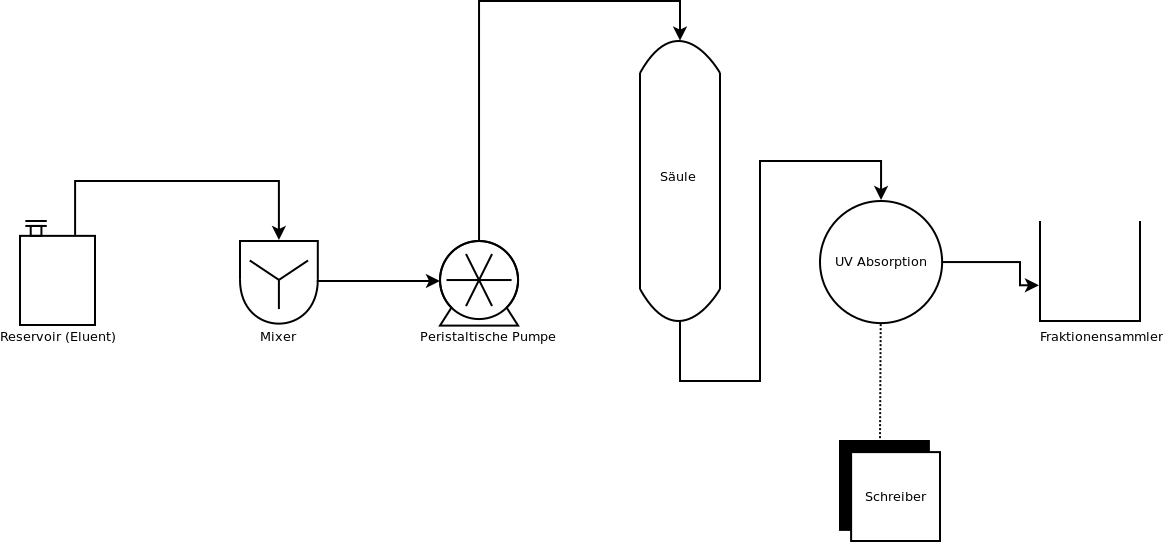
\includegraphics[width=0.9\textwidth]{img/apparatur.png}
	\caption{Apparatur für Ionenaustauschchromatographie}
	\label{fig:apparatur}
\end{figure}

Abbildung \ref{fig:apparatur} ist eine systematische Darstellung der
verwendeten Versuchsapparatur, mit welcher die Ionenaustauschchromatographie
durchgeführt wurde.

\chapter{Material \& Chemikalien}

\section{Material}

\begin{itemize}
	\item 1 Styroporbox mit Eis
	\item Schnitzer und Kartoffeln
	\item 1 Mixer
	\item 1 Sorvallzentrifuge und SS34 Rotor
	\item 2 Sorvallzentrifugen-Röhrchen
	\item 1 \SI{500}{ml}, 2 \SI{100}{ml} Becherglas
	\item 2 \SI{500}{ml} Duran Flaschen
	\item 1 Säule
	\item 1 Peristaltische Pumpe
	\item 1 Fraktionensammler
	\item 1 UV-Detektor
	\item 1 Schreiber
	\item 1 Magnetrührer
	\item 1 kleiner linearer Gradientenmischer
	\item 1 Mikrotiterplatte
	\item 1 12-Kanalpipette mit Spitzen
\end{itemize}

\section{Chemikalien \& Lösungen}

\begin{itemize}
	\item  \SI{1}{\Molar} \ce{TRIS-HCl}, pH 7.75
	\item \ce{NaCl}
	\item Puffer A: \SI{20}{\milli\Molar} \ce{TRIS-HCl}, pH 7.75
	\item Puffer B, Eluent: Puffer A + \SI{1}{\Molar} \ce{NaCl}
	\item ABTS-Stocklösung in \ce{H2O}, \SI{50}{\milli\gram \per \milli\litre}
	\item Horse radish peroxidase, HR-POX: Aktivität ca \SI{700}{U \per \milli\gram}
	\item Bovine liver catalase: Aktivität \SI{2088}{U \per \milli\gram}
	\item \ce{H2O2} \SI{30}{\percent} in \ce{H2O}
	\item Magermilchpulver
\end{itemize}

\cite{skriptv9}

\chapter{Durchführung}

\section{Vorbereitung Lösungen}

Basierend auf \SI{1}{\Molar} \ce{TRIS-HCl} Stocklösung, und \ce{NaCl}
(Molekulargewicht \SI{58.443}{\gram\per mol} Herstellung von:
\begin{itemize}
	\item \SI{500}{ml} Puffer A, \SI{20}{\milli\Molar} \ce{TRIS-HCl}: \SI{10}{\ml} \ce{TRIS-HCl} in Wasser
	\item \SI{500}{ml} Puffer A, \SI{20}{\milli\Molar} \ce{TRIS-HCl} \& \SI{1}{\Molar} \ce{NaCl}: \SI{10}{\ml} \ce{TRIS-HCl} in Wasser \& \SI{29.22}{\g} \ce{NaCl}
\end{itemize}

\section{Vorbereitung Säule}

\begin{itemize}
	\item Säule vorgängig ausgespült
	\item Zugabe von \SI{3}{ml} Säulenmaterial in Puffer
	\item Sobald Material gesetzt, Ablass Puffer bis noch \SI{1}{cm} über Säulenmaterial
\end{itemize}

\section{Herstellung Kartoffelextrakt}

Herstellung des Kartoffelextrakts durch eine der Gruppen für beide Gruppen.

\begin{itemize}
	\item Drei Kartoffeln gewaschen und gewürfelt
	\item \SI{150}{g} Kartoffeln mit \SI{150}{ml} Puffer A in Mixer homogenisiert
	\item Überstand in Zentrifuge bei 10000 RPM für \SI{10}{min} zentrifugiert
	\item Klarer Überstand unter Vakuum abfiltriert
	\item \SI{30}{ml} Filtrat je Gruppe auf Eis aufbewahrt
	\item $\text{OD}_{280}$ einer 1:20 Verdünnung der Extraktlösung, sowie
		des TRIS-Puffers als Referenz, bestimmt. $\text{OD}_{280} =
		\SI{0.688}{\mg \per \ml}$
	\item Damit Proteinkonzentration des Extrakts $\SI{0.688}{\mg \per \ml}
		\cdot 20 = \SI{13.76}{\mg \per \ml}$.
\end{itemize}

\section{Vorbereitung UV-Detektor, Schreiber, Fraktionensammler}

In Voraus durch Assistenten bereitgestellt.

\section{Ionenaustauschchromatographie}

\begin{itemize}
	\item Pumpe auf \SI{2}{\ml \per \min} eingestellt
	\item Fraktionensammler \& Schreiber gestartet
	\item 8 Fraktionen (8 Minuten) lang Säule mit Puffer A äquilibriert
	\item \SI{4.36}{ml} Extrakt (entspricht \SI{60}{mg} Proteinen,
		vergleiche Berechnung oben) auf Säule geladen
	\item Sobald alles Extrakt geladen, wieder Wechsel auf Puffer A
	\item Mit Pufferlösung weitergewaschen bis Basislinie des UV-Detektors
		wieder erreicht (dH alles Protein entweder gebunden in Säule,
		oder ausgewaschen)
	\item Bei Fraktion 31 Reservoir auf Puffer B gewechselt. Durch den
		Mixer wurde somit ein linearer Elutions-Gradient erzeugt.
	\item Während Elution zweimal manuelle Korrektur des Schreibers
		notwendig, aufgrund eines technischen Versagens in dem der
		Schreiber auf die Null-Linie zurückfiel.
	\item Nach erfolgter Elution Schreiber, Fraktionensammler und Pumpe gestoppt.
\end{itemize}

\section{Vorbereitung Mikrotiterplatte}

Durch andere Gruppe Mikrotiterplatte mit Proteinen gesättigt, gewaschen und
getrocknet.

\section{Vorbereitung Reagenzien für Mikrotiterplatten-Assay}

\begin{itemize}
	\item Durch andere Gruppe \SI{0.001}{\percent} \ce{H2O2} Lösung in Puffer A hergestellt
	\item Herstellung \SI{10}{ml} HR-POX Assaystammlösung mit \SI{0.05}{\mg
		\per \ml} HR-POX, \SI{1}{\mg \per \ml} ABTS, aus:
		\begin{itemize}
			\item \SI{9.3}{\ml} Puffer A
			\item \SI{500}{\ul} HR-POX Stocklösung (\SI{1}{\mg \per \ml})
			\item \SI{200}{\ul} ABTS (\SI{50}{\mg \per \ml})
		\end{itemize}
\end{itemize}

\section{Mikrotiterplatten-Assay}

\begin{itemize}
	\item Auswahl von 7 Fraktionen der Gradientenelution: G36, G38, G40,
		G42, G44, G46, G48
	\item Vorlegen von \SI{50}{\ul} \SI{20}{\milli\Molar} Puffer A in
		Reihen B bis H der Platte
	\item \SI{100}{\ul} Puffer A als Negativkontrolle in A1
	\item \SI{100}{\ul} Katalase-Lösung in A2
	\item \SI{100}{\ul} Rohextrakt in A3
	\item A4 leergelassen da 12-Kanalpipette dort defekt
	\item \SI{100}{\ul} einer Fraktion des Durchlaufes in A5
	\item \SI{100}{\ul} der Fraktionen der Elution in A6 bis A12
	\item Lösungen in Reihe A Seriell 1:1 in Reihen B bis H verdünnt.
	\item Von Reihe H nach A Zugabe \SI{50}{\ul} der vorbereiteten
		\ce{H2O2} Lösung
	\item Nach 15 Minuten von Reihe A nach H Zugabe von \SI{50}{\ul} der
		vorbereiteten HR-POX Lösung
	\item Beobachtung der Farbumschläge, Abschätzung der
		Katalase-Konzentrationen in einzelnen Fraktionen
	\item Platte gewaschen und getrocknet
\end{itemize}

\section{Ionenaustauschchromatographie in automatischer Säule}

Durch Assistent durchgeführt:

\begin{itemize}
	\item Vier Fraktionen mit höchster Katalase-Aktivität kombiniert
	\item In Zentrifuge mehrfach gefiltert
	\item Filterrückstand in Puffer gelöst, in Säule aufgetrennt und
		UV-Absorption gemessen
\end{itemize}

\chapter{Resultate}

\section{UV-Absorptionsmessung während Ionenaustauschchromatographie}

\begin{figure}[h]
	\centering
	\includegraphics[width=0.9\textwidth]{img/chromatographie_graph.png}
	\caption{UV-Absorption während Ionenaustauschchromatographie}
	\label{fig:chrom_graph}
\end{figure}

In Abbildung \ref{fig:chrom_graph} ist der vom Schreiber geplottete Wert der
UV-Absorptionsmessung während der Chromatographie ersichtlich. Die Vertikalen
Balken markieren den Zeitpunkt von wichtigen Aktionen, die Zahlen am oberen
Rand bezeichnen die Fraktionen.

In einer ersten Phase wurde die Säule mit Puffer A gespült, der
Absorptions-Wert blieb dabei, wie erwartet, tief und konstant. Nach Fraktion 8
wurde das Protein via Pumpe zugegeben.

Ab Fraktion 12 beginnt der Durchlauf mit dem klar ersichtlichen
Durchlaufpeak. Hier passierten alle Proteine, die nicht an die Säule binden
konnten, den Detektor. Dies waren sowohl Proteine die aufgrund ihrer fehlenden
negativen Ladung nicht an die Säule binden konnten, wie auch - was später
ersichtlich sein wird - negativ geladene Proteine die wegen zu hoher
Proteinkonzentration nicht an die Säule binden konnten.

Sobald die Messwerte wieder die Basislinine erreicht hatten, wurde nach
Fraktion 30 auf einen linearen Gradienten mit Puffer B gewechselt. Während der
Elution sind zwei grosse und ein kleiner Peak ersichtlich, in jenem bestimmte
Proteine - oder Gruppen von Proteinen - aufgrund der aktuellen Konzentration
des Eluenten aus der Säule gelöst wurden.

Während der Elution fiel der Schreiber aufgrund eines technischen Defekts auf
die Nulllinie zurück und musste zu zwei darauffolgenden Zeitpunkten manuell
eingestellt werden,was zu den sichtbaren Sprüngen führte.

\section{Katalase-Nachweis}

\begin{figure}[h]
	\centering
	\includegraphics[width=0.9\textwidth]{img/mikrotiterplatte.png}
	\caption{Mikrotiterplatten Assays zwecks Katalase-Nachweis}
	\label{fig:katalase_nachweis}
\end{figure}

In Abbildung \ref{fig:katalase_nachweis} ist die in der Einleitung erwähnte
Reaktion mit einhergehender Farbveränderung beobachtbar. Wie eingangs erwähnt
bedeutet die grüne Farbe, dass keine Katalase vorhanden war wohingegen in
farblosen Lösungen Katalase vorhanden war.

Wie erwartet ist die Negativprobe mit Puffer A konstant grün. Die Positivprobe
mit einer Katalasen-Lösung bekannter Konzentration verhält sich ebenso wie
erwartet, insofern dass die abnehmende Katalasenkonzentration in der
Verdünnungsreihe dazu führt, dass die Probe grüner wird.

Aus dem Farbverlauf der Verdünnungsreihe des Rohextrakts lässt sich schliessen,
dass im Rohextrakt Katalase vorhanden ist. Das gleiche gilt für die
Verdünnungsreihe des Durchlaufs, was darauf hindeutet, dass die zugegebene
Proteinkonzentration zu hoch für die Säule war und gewisse Katalase nicht an
die Säule binden konnte.

Aus dem Farbverlauf der Verdünnungsreihen der Fraktionen der Elution ist
ersichtlich, dass die Mehrheit der Katalase in den Fraktionen 42-48 ist. Dies
sind jene Fraktionen die direkt im Anschluss an den grössten Elutionspeak
folgten, was andeutet, dass die Katalase bei jener Konzentration des Eluenten
gelöst wurde.

\subsection{Quantitativer Vergleich der Katalase-Konzentration}

In jenen Fraktionen der Elution in welchen Katalase nachweisbar war, wurde
jeweils die am stärksten verdünnte, noch vom Nachfolger unterscheidbare, Lösung
bestimmt, und deren Farbe mit der der bekannten Positivprobe verglichen.  Somit
liess sich die Konzentration in jener Lösung abschätzen, und aufgrund der
bekannten seriellen Verdünnungsreihe jene der unverdünnten Fraktion herleiten.
Hieraus ergaben sich folgende Konzentrationen für die einzelnen Reihen, wobei
`-' die Negativprobe, `+' die Katalase-Lösung bekannter Konzentration, `R' das
Rohextrakt, und `D' die Fraktion des Durchlaufs ist. `36' bis `48' sind die
bekannten Fraktionen der Gradientenelution. Leere Felder bedeuten, dass keine
Katalase-Aktivität nachgewiesen werden konnte. Alle Konzentrationen sind in
\si{\ug \per \ml}.
\\

\begin{tabu}{cccccccccccc}
	\toprule
	- & +      & R      & & D      & 36 & 38    & 40    & 42     & 44    & 46    & 48    \\
	\midrule
	  & 10     & 20     & & 10     &    & 0.313 & 0.625 & 1.25   & 1.25  & 1.25  & 1.25  \\ 
	  &  5     & 10     & &  5     &    & 0.156 &       & 0.625  & 0.625 & 0.625 & 0.625 \\ 
	  &  2.5   &  5     & &  2.5   &    &       &       & 0.313  & 0.313 & 0.313 & 0.313 \\ 
	  &  1.25  &  2.5   & &  1.25  &    &       &       &        &       &       &       \\ 
	  &  0.625 &  1.25  & &  0.625 &    &       &       &        &       &       &       \\ 
	  &  0.313 &  0.625 & &  0.313 &    &       &       &        &       &       &       \\ 
	  &  0.156 &  0.313 & &  0.156 &    &       &       &        &       &       &       \\ 
	  &  0.078 &  0.156 & &        &    &       &       &        &       &       &       \\ 
	\bottomrule
\end{tabu}

\section{Chromatographie in automatischer Säule} 

\begin{figure}[h]
	\centering
	\includegraphics[width=0.9\textwidth]{img/chromatographie_auto_graph.png}
	\caption{UV-Absorption während Ionenaustauschchromatographie in Äkta}
	\label{fig:chrom_graph_auto}
\end{figure}

In Abbildung \ref{fig:chrom_graph_auto} sind die Resultate der
Nachmittags-Messung auf der `Äkta' Säule ersichtlich. Interessant ist der
Bereich ab \SI{0}{s}, die Messungen vorher sind während dem automatischen
Spülen der Maschine. Der grüne Graph stellt die Konzentration des Puffer B dar,
der blaue die Absorption des UV-Detektors, und der braune die Ionen-Konzentration.

Zum Zeitpunkt \SI{0}{s} werden die Proteine in die Säule geladen, und kurz
darauf steigt die Ionenkonzentration im Ausgang leicht an. Dies deutet darauf
hin, dass das verwendete Proteingemisch nicht komplett rein war, und
gewisse positiv geladenen Proteine vorhanden waren, welche nicht an die Säule
binden konnten. Dies entspricht dem Durchlauf-Peak der Messung am Vormittag,
wenn auch bedeutend kleiner, da das Gemisch bereits mehrfach gereinigt wurde.

Während der Elution sind beim UV-Detektor zwei Peaks ersichtlich. Dies
impliziert, dass im Proteingemisch mindestens zwei Proteine vorhanden waren,
die unterschiedlich stark an die Säule banden. Da die Peaks zusätzlich nicht
sauber getrennt sind, wird in den einzelnen Fraktionen keine saubere Trennung
der beiden Proteingruppen vorhanden sein. Wäre dies gewünscht, könnte die
Maschine so konfiguriert werden, dass sie beim ersten Peak die Konzentration
des Puffer B eine Weile hält, bis die erste Gruppe an Proteinen ausgewaschen
ist.

Sobald die Puffer-Konzentration das Maximum erreicht hat, und keine weitere
Proteine ausgewaschen werden, beendet die Maschine ebenfalls.

\chapter{Diskussion}

\section{Anzahl Peaks}

In der am Morgen durchgeführten Chromatographie sind vier Peaks ersichtlich.
Der erste grosse Peak ist der Durchlaufpeak, in dem alle Proteine welche nicht
negativ geladen sind und somit nicht an die Säule binden, wie auch alle
Proteine die aufgrund der zu hohen Proteinkonzentration nicht binden konnten,
den Detektor passieren.

Während der Elution sind drei Peaks ersichtlich, was darauf hindeutet, dass
mindestens drei negativ geladene, unterschiedlich stark an die Säule bindende,
Proteine im Rohextrakt vorhanden sind.

Aus der schlechten Trennung der Peaks lässt sich auch ableiten, dass die
Proteine in den Fraktionen schlecht getrennt sein werden. Wäre eine bessere
Trennung erwünscht, wäre ein langsamerer, oder stärker kontrollierte, Gradient nötig

\section{Reihenfolge der Zugabe \ce{H2O2} \& HR-POX zu Assay}

Die vorgegeben Reihenfolge verhindert, dass die Assays durch unsauberes
Arbeiten verunreinigt werden, ohne dass zwischen jeder Reihe die Spitzen
gewechselt werden müssen.

Bei der Zugabe von \ce{H2O2} wird entlang der aufsteigenden
Katalase-Konzentration gearbeitet, um keine Katalase aus den höher
Konzentrierten Proben in die tiefer Konzentrierten einzuschleppen. Bei der
Zugabe von HR-POX wird entlang der erwarteten aufsteigenden \ce{H2O2}
Konzentration gearbeitet, um nicht \ce{H2O2} in jene Proben einzuschleusen, in
welchen sie durch die Katalase abgebaut wurde.

\section{Fraktionen mit Katalase}

Wie oben erwähnt, kann Katalase in den folgenden Fraktionen nachgewiesen
werden:

\begin{itemize}
	\item Durchlauf: Was impliziert dass die Protein-Konzentration zu hoch
		für die gegebene Säulenkapazität gewählt wurde
	\item Rohextrakt: Was zu erwarten war
	\item Positiv-Probe: Was zu erwarten war
	\item Mehreren Fraktionen der Elution
\end{itemize}

\section{Abschätzung der Katalasen-Konzentration in den Fraktionen}

Im Bezug auf die obenstehenden Rechnungen folgen folgende Konzentrationen:
\begin{itemize}
	\item Rohextrakt: \SI{20}{\ug \per \ml}
	\item Durchlauf: \SI{10}{\ug \per \ml}
	\item Fraktion 38: \SI{0.313}{\ug \per \ml}
	\item Fraktion 40: \SI{0.625}{\ug \per \ml}
	\item Fraktion 42: \SI{1.25}{\ug \per \ml}
	\item Fraktion 44: \SI{1.25}{\ug \per \ml}
	\item Fraktion 46: \SI{1.25}{\ug \per \ml}
	\item Fraktion 48: \SI{1.25}{\ug \per \ml}
\end{itemize}

Diese Zahlen erscheinen plausibel, da die Summe der Konzentrationen aus
Durchlauf und Fraktionen ungefähr der Konzentration im Rohextrakt entspricht -
die Differenz lässt sich mit der Ungenauigkeit der
Konzentrations-Abschätzung erklären.

\section{Aufreinigung vs Anreicherung}

Durch den Anionentauscher in der ersten Chromatographie wurden alle ungeladenen
sowie positiv geladenen Proteine im Durchlauf ausgespült, und die Konzentration
von Fremdproteinen so bereits stark gesenkt. Damit kann - verglichen mit einer
Anreicherung bei der lediglich die Konzentration der Katalase erhöht worden
wäre - bereits von einer Aufreinigung gesprochen werden.

Klar ist aber auch, dass das resultierende Proteingemisch noch nicht rein ist.
Ersichtlich ist dies beispielsweise daran, dass in der zweiten Chromatographie
am Nachmittag zwei Peaks ersichtlich waren - also mindestens zwei Proteine im
Gemisch vorhanden bleiben. Je nach Verwendungszweck wäre eine weitere
Aufreinigung notwendig.

\section{Katalase-Nachweis via Mikrotiterplatten-Assay im Vergleich mit Alternativen}

Eine weitere Möglichkeit, Katalase-Aktivität nachzuweisen, ist via die
Produktion von Sauerstoff beim Abbau von \ce{H2O2} durch Katalase. Dieser
Sauerstoff führt beispielsweise zur Schaumbildung in einem Reagenzglas mit
Probematerial, oder führt auch dazu, dass ein eingetauchter Glimmspan merklich
stärker leuchtet.

Diese Schaumbildung kann so nicht nur zum Nachweis hergezogen werden, sondern
auch beispielsweise zum Vergleich der Katalase-Aktivität zweier Proben.

Der Vorteil jener Methode ist, dass keinerlei zusätzlichen - potentiell teuren
- Chemikalien für Nachweiszwecke notwendig sind. Dafür können mit
Mikrotiterplatten-Assays viele Proben gleichzeitig, und mit kleinen Mengen an
Stoff je Probe, untersucht werden. Auch ist die quantitative Aussage
zuverlässiger, als die Konzentration der Katalase via Höhe des gebildeten
Schaumes abzuschätzen.

\bibliographystyle{plain}
\bibliography{references}

\end{document}
